\documentclass{article}

\usepackage[spanish]{babel}
\usepackage{amsmath}
\usepackage{graphicx}
\usepackage{geometry}
\usepackage{float}
\usepackage[urlcolor=blue]{hyperref}
\usepackage{titlesec}
\usepackage{titling}

\geometry{
    top = 2cm, 
    bottom = 2cm, 
    left = 2cm, 
    right = 2cm, 
}

\title{Tarea 1 Metodos no Param\'etricos \\
github:}
\author{Rudy Miranda}
\date{abril, 2023}

\begin{document}
    \maketitle
    \tableofcontents

    \section{Introducci\'on}

    Se nos presenta una pequena base de datos referente a 100 empresas, las cuales presentan 4 variables cada una; 2 cualitativas (origen y tipo), y las restantes cuantitativas (tiempo y capitazaci\'on).

    Luego de un an\'alisis exploratorio realizaremos dos pruebas no param\'etricas. La primera sera la prueba de Kolmogorov-Smirnov para el an\'alisis de normalidad, seguido de una prueba de signos para una mediana propuesta.
    
    \section{An\'alisis Exploratorio}

    \subsection{Variables Categoricas}
    
    \begin{center}
        \begin{minipage}{0.6\linewidth}
            \begin{minipage}{0.45\linewidth}
                \begin{figure}[H]
                    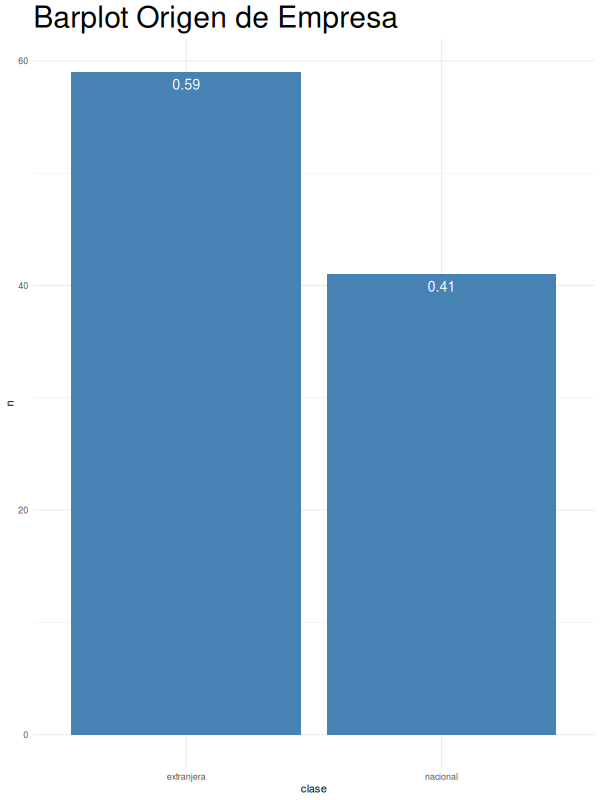
\includegraphics[width=\linewidth]{../bar1.png}
                \end{figure} 
            \end{minipage}
            \hspace{0.05\linewidth} 
            \begin{minipage}{0.45\linewidth}
                \begin{figure}[H]
                    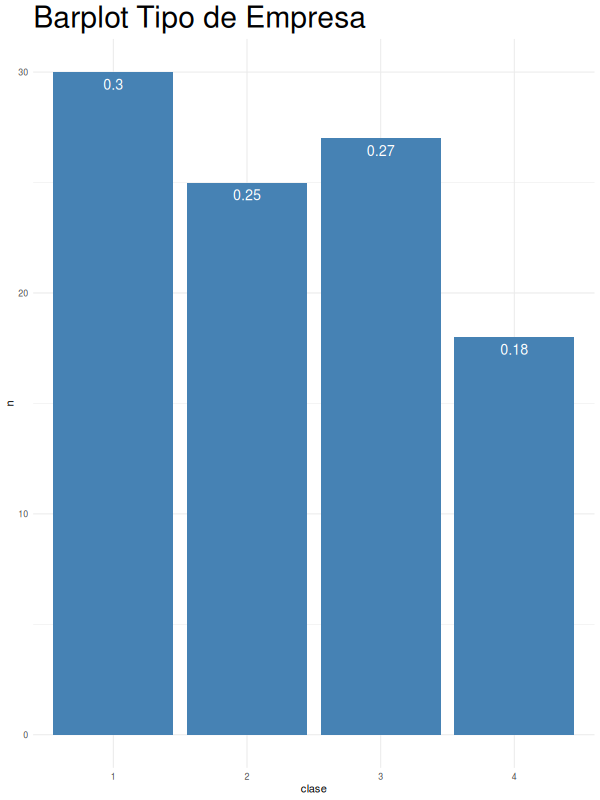
\includegraphics[width=\linewidth]{../bar2.png}
                \end{figure} 
            \end{minipage}
        \end{minipage}
    \end{center}

    \subsection{Variables Cuantitativas}

    \begin{table}[H]
        \centering
        \begin{tabular}{lll}
            & Tiempo & Capitalizaci\'on \\ \cline{2-3} 
            \textit{mean}     & 3.176  & 11.695         \\
            \textit{sd}       & 3.821  & 9.658          \\
            \textit{min}      & 0      & 0.1            \\
            \textit{max}      & 18.4   & 46.18          \\
            \textit{skewness} & 1.898  & 1.587          \\
            \textit{kurtosis} & 6.61   & 5.543         
        \end{tabular}
    \end{table}

    \section{Test de Normalidad Variable Capitalizaci\'on}

    \begin{center}
        \begin{minipage}{0.9\linewidth}
            \begin{minipage}{0.45\linewidth}
                \begin{figure}[H]
                    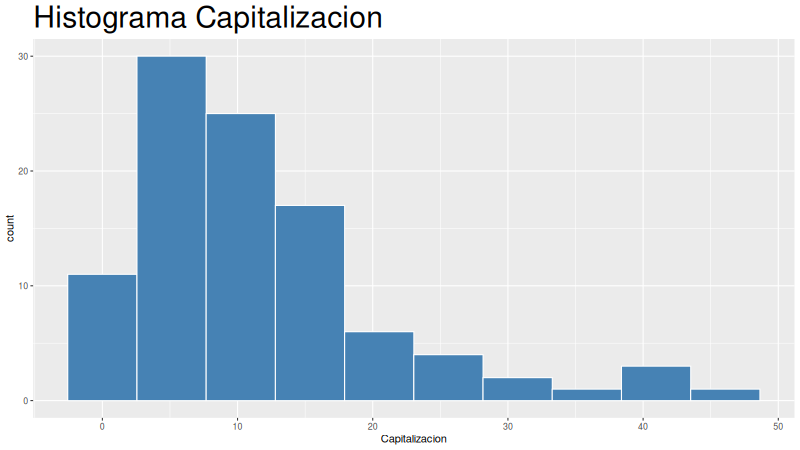
\includegraphics[width=\linewidth]{../hist2.png}
                \end{figure} 
            \end{minipage}
            \hspace{0.05\linewidth} 
            \begin{minipage}{0.45\linewidth}
                \begin{figure}[H]
                    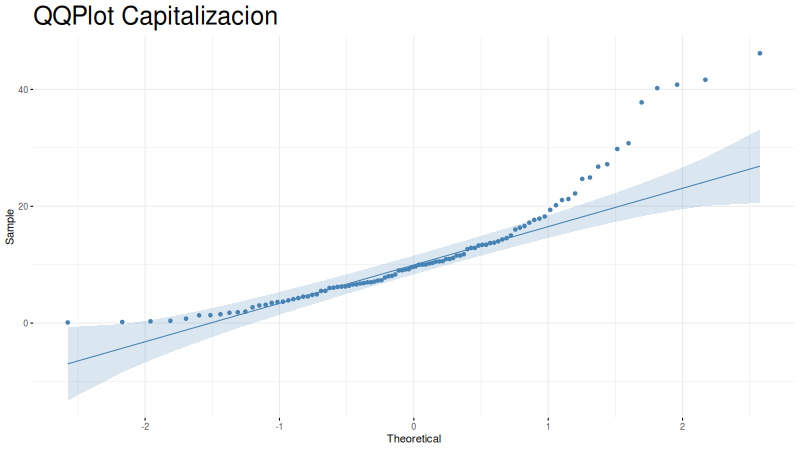
\includegraphics[width=\linewidth]{../qqplot.png}
                \end{figure} 
            \end{minipage}
        \end{minipage}
    \end{center}
    
    En primera instancia notamos que tanto por la kurtosis y coeficiente de asimetr\'ia, ademas del histograma y el \textit{QQplot}, que no estamos en presente de una variable aleatoria que se distribuya normal.

    Para formalizar esta afirmaci\'on la respaldaremos el test de normalidad no param\'etrico de Kolmogorov-Smirnov.

    \subsection{Test de Kolmogorov-Smirnov}

    Proponemos las hip\'otesis

    \begin{center}
        $H_0: X_{\text{Capitalizaci\'on}} \sim N(\mu, \sigma^2)$ \text{ vs } $H_1: X_{\text{Capitalizaci\'on}} \not\sim N(\mu, \sigma^2)$
    \end{center}

    el estad\'istico de prueba en este caso es

    \begin{equation}
        D = \max\limits_{1\leq i \leq n} = \left\{D^{+}, D^{-}\right\}
    \end{equation}
    
    Donde los 
    \begin{align}
        D^{+} &= \Big| \frac{i}{n} - F_0 (x_i) \Big| \\
        D^{-} &= \Big| F_0 (x_i) - \frac{i - 1}{n} \Big| 
    \end{align}

    nuestra region de rechazo para $D$ seria

    \begin{equation}
        \left] D_\alpha, +\infty \right[
    \end{equation}

    Donde, para un nivel de confianza del 0.95, y nuestra cantidad de datos (100)
    
    \begin{align}
        D_\alpha &= \frac{C_\alpha = 0.895}{K(n) = \sqrt{100} - 0.01 + \frac{0.85}{\sqrt{100}}} \\
                 &= 0.089
    \end{align}

    Con la funci\'on nativa de \textit{R}, \textit{ks.test}, obtenemos que el valor del estad\'istico $D = 0.146$. Por lo anterior rechazamos $H_0$, ya que pertenece a la region de rechazo.
    
    \section{Test de Normalidad Variable Tiempo}
    
    \begin{center}
        \begin{minipage}{0.9\linewidth}
            \begin{minipage}{0.45\linewidth}
                \begin{figure}[H]
                    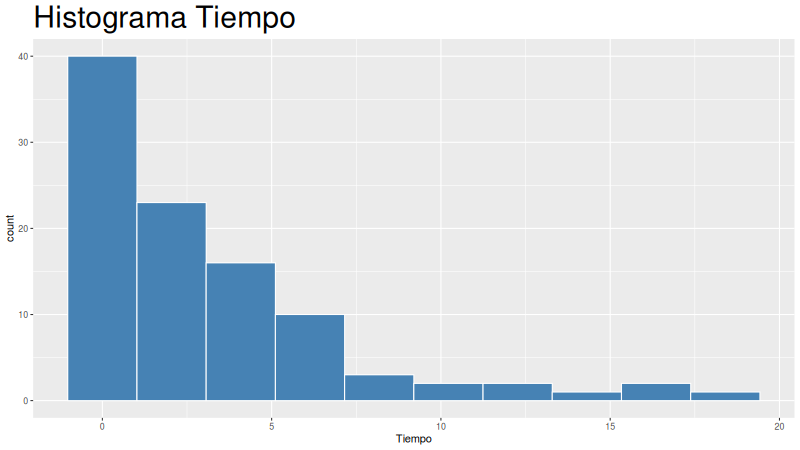
\includegraphics[width=\linewidth]{../hist1.png}
                \end{figure} 
            \end{minipage}
            \hspace{0.05\linewidth} 
            \begin{minipage}{0.45\linewidth}
                \begin{figure}[H]
                    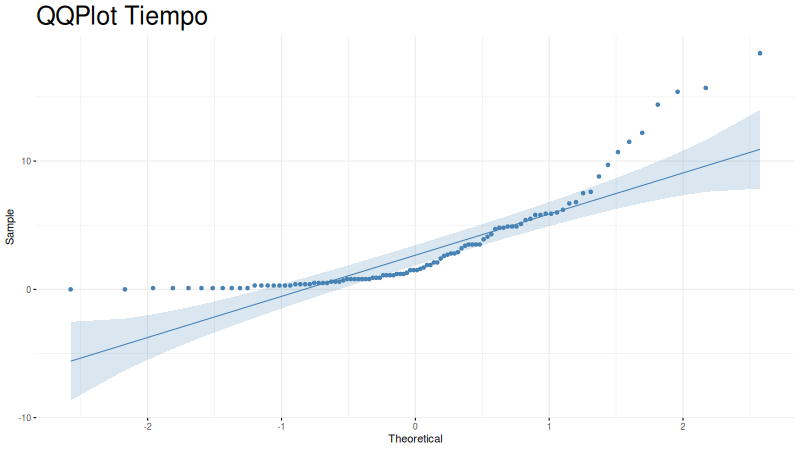
\includegraphics[width=\linewidth]{../qqplot1.png}
                \end{figure} 
            \end{minipage}
        \end{minipage}
    \end{center}
    En este caso seremos mas breves, ya que el procedimiento es el mismo que con la variable anterior.
    
    Proponemos las siguientes hip\'otesis
    \begin{center}
        $H_0: X_{\text{Tiempo}} \sim N(\mu, \sigma^2)$ \text{ vs } $H_1: X_{\text{Tiempo}} \not\sim N(\mu, \sigma^2)$
    \end{center}

    En este caso el valor de nuetro estad\'istico $D = 0.203$, y el valor critico $D_\alpha = 0.089$. Nuevamente se rechaza la hipotesis nula, al ser $D > D_\alpha$.
    
    \section{Capitalizaci\'on Mediana de Empresas Nacionales}

    Proponemos las hip\'otesis
    \begin{center}
        $H_0: m = 10.5 \text{ vs } H_1: m \neq 10.5$
    \end{center}
    donde $m$ corresponde a la mediana poblacional.

    El test a usar sera el de los signos, en el cual el estad\'istico de prueba es

    \begin{equation}
        r = \max\limits_{1\leq i\leq n} \left\{ r^{+}, r^{-}\right\}
    \end{equation}

    Donde

    \begin{align}
        r^{+} &= \text{cantidad de observaci\'on por sobre la mediana propuesta} \\
        r^{-} &= \text{cantidad de observaci\'on bajo la mediana propuesta} \\
            n &= \text{cantidad de observaciones(41)}
    \end{align}
    
    un inconveniente con este test es que require descartar las observaciones iguales a la mediana propuesta, pero no es el caso de nuestros datos, por lo que no debemos disminuir nuetro tamano muestral.

    Al calcular $r^{+}$ y $r^{-}$ (18 y 23 respectivamente), obtenemos el valor de nuestro estad\'istico $r = 23$.

    Finalmente podemos conocer el valor-$p$, ya que sabemos que $r \sim B(41, 0.5)$, entonces

    \begin{equation}
        p = 2 * P(r > 23 ) = 0.53
    \end{equation}

    Dado que $p > \alpha = 0.05$, no hay evidencia suficiente para rechazar la hip\'otesis nula.
\end{document}
